\section{Similarly ordered four-element sets}\label{sec:similar}\label{subsec:similar}

This section proves Theorem~\ref{thm:B}. For four elements the residue pairs of Section~\ref{sec:sumsets} at $m=d$ come from a two-dimensional diagram of $d$ lattice points, and similar ordering becomes a condition on its layers that can be checked from the two Ap\'ery sets.


Let $A_0=\{0,a_1,a_2,d\}$, $0<a_1<a_2<d$. Let $w^{(1)}_r$ and $w^{(2)}_r$ be the Ap\'ery elements of $S_1$ and $S_2$ modulo $d$, as in Section~\ref{subsec:counting} with $m=d$ (subscripts modulo $d$), and for $0\le r<d$ put
\begin{equation}\label{eq:diagram}
t_r=\frac{w^{(1)}_r+w^{(2)}_{-r}}{d},\qquad y_r=\frac{w^{(1)}_r-a_1t_r}{a_2-a_1},\qquad x_r=t_r-y_r .
\end{equation}

\begin{lemma}[Common diagram]\label{lem:diagram}
A four-element set is CM if and only if all $x_r,y_r$ are nonnegative integers. Then $\mathcal D=\{(x_r,y_r):0\le r<d\}$ consists of $d$ points, it is an order ideal of $\N^2$, the point $(x,y)$ of residue $r$ satisfies $w^{(1)}_r=a_1x+a_2y$ and $w^{(2)}_{-r}=(d-a_1)x+(d-a_2)y$, and with $s=-r\bmod d$,
\begin{equation}\label{eq:uv-diagram}
u_s=\Bigl\lceil\frac{a_1x+a_2y}{d}\Bigr\rceil,\qquad v_s=x+y-u_s .
\end{equation}
\end{lemma}

\begin{proof}
The point $(w^{(1)}_r,w^{(2)}_{-r})$ lies in $G\cap(S_1\times S_2)$ and is the coordinatewise least point there with first coordinate $\equiv r$. If $A_0$ is CM it lies in $\mathcal S$ (Theorem~\ref{thm:cm}); a representation cannot use $(d,0)$ or $(0,d)$, by minimality of $w^{(1)}_r$ and $w^{(2)}_{-r}$, so it is $x(a_1,d-a_1)+y(a_2,d-a_2)$, and solving gives $(x,y)=(x_r,y_r)$. Conversely, if the $x_r,y_r$ are nonnegative integers, every point of $G\cap(S_1\times S_2)$ is some $(w^{(1)}_r,w^{(2)}_{-r})\in\mathcal S$ plus multiples of $(d,0)$ and $(0,d)$, so $A_0$ is CM. If $(x',y')\le(x,y)\in\mathcal D$ and an element of $S_1$ smaller than $a_1x'+a_2y'$ were in its class, adding $a_1(x-x')+a_2(y-y')$ would contradict the minimality of $a_1x+a_2y$; the same holds for $S_2$, so $(x',y')\in\mathcal D$. Finally $u_s=(d-r+w^{(1)}_r)/d=\lceil w^{(1)}_r/d\rceil$ for $r>0$, and $u_s+v_s=t_r$.
\end{proof}

For $(x,y)\in\N^2$ call $a_1x+a_2y$ and $(d-a_1)x+(d-a_2)y$ its two values and $a_1x+a_2y\bmod d$ its residue. For a nonempty layer $\mathcal D_t=\{(x,y)\in\mathcal D:x+y=t\}$ let $F^-_t$ and $F^+_t$ be the least and largest values of $a_1x+a_2y=a_1t+(a_2-a_1)y$ on it, attained at the least and largest $y$.

\begin{theorem}[Similar ordering]\label{thm:similar}
For a CM set $\{0,a_1,a_2,d\}$ the following are equivalent:
(1) $(u,v)$ is similarly ordered at $m=d$;
(2) $\lceil(a_1x+a_2y)/d\rceil$ is constant on each layer $\mathcal D_t$;
(3) $\lceil F^-_t/d\rceil=\lceil F^+_t/d\rceil$ for every nonempty layer, that is, each layer is mapped into one interval $((q-1)d,qd]$ with $q\in\Z$.
\end{theorem}

\begin{proof}
By \eqref{eq:uv-diagram} two points of $\mathcal D_t$ give pairs $(u,t-u)$, $(u',t-u')$, incomparable if $u\ne u'$; so (1) implies (2). Assume (2), with value $q_t$ on $\mathcal D_t$. The nonempty layers are $0,\dots,t^*$, and every point of layer $t+1$ lies above a point of layer $t$ whose value $a_1x+a_2y$ is smaller by $a_1$ or $a_2\in(0,d)$, so $q_{t+1}-q_t\in\{0,1\}$. Hence $q_t$ and $t-q_t$ are nondecreasing and the pairs $(q_t,t-q_t)$ form a chain. (2) and (3) are equivalent because the value increases with $y$ on a layer.
\end{proof}

\begin{proposition}[Shape]\label{prop:shape}
For a CM set $\{0,a_1,a_2,d\}$, $\mathcal D$ is a rectangle $[0,P-1]\times[0,Q-1]$ or an L-shape $([0,W-1]\times[0,Q-1])\cup([W,P-1]\times[0,Z-1])$ with $0<W<P$, $0<Z<Q$, and then $a_1W+a_2Z\equiv0\pmod d$. If $P-W\ge2$ and $Q-Z\ge2$, $(u,v)$ is not similarly ordered.
\end{proposition}

\begin{proof}
The minimal points of $\N^2\setminus\mathcal D$ are $(P,0)$, $(0,Q)$ and possibly points $(p,q)$ with $p,q>0$. For such a point let $(x,y)\in\mathcal D$ be the point of its residue; its two values are at most those of $(p,q)$, one strictly. If $x>0$, then $(p-1,q)\in\mathcal D$ while $(x-1,y)$ has the same residue and values at most those of $(p-1,q)$, one strictly, contradicting Lemma~\ref{lem:diagram}; similarly if $y>0$. So $(x,y)=(0,0)$ and $a_1p+a_2q\equiv0$. Two such points $(p_1,q_1)$, $(p_2,q_2)$ with $p_1<p_2$ would put the distinct points $(p_2-p_1,0)$ and $(0,q_1-q_2)$ of the same residue in $\mathcal D$ (as $p_2-p_1<P$ and $q_1-q_2<Q$). If $P-W,Q-Z\ge2$, the points $(W\mp1,Z\pm1)$ lie on one layer with values $a_1W+a_2Z\pm(a_2-a_1)$ around a positive multiple of $d$, and Theorem~\ref{thm:similar} applies.
\end{proof}

That $\mathcal D$ is a rectangle or an L-shape is the classical shape of the Ap\'ery set of the three-generated semigroup $S_1=\langle a_1,a_2,d\rangle$ with respect to $d$, drawn in the coordinates of $a_1$ and $a_2$ \cite{AguiloMarijuan2014}; what is used here is the congruence of the notch and its consequence for similar ordering. Figure~\ref{fig:diagrams} shows the test of Theorem~\ref{thm:similar} on two sets of the introduction.

\begin{figure}[ht]
\centering
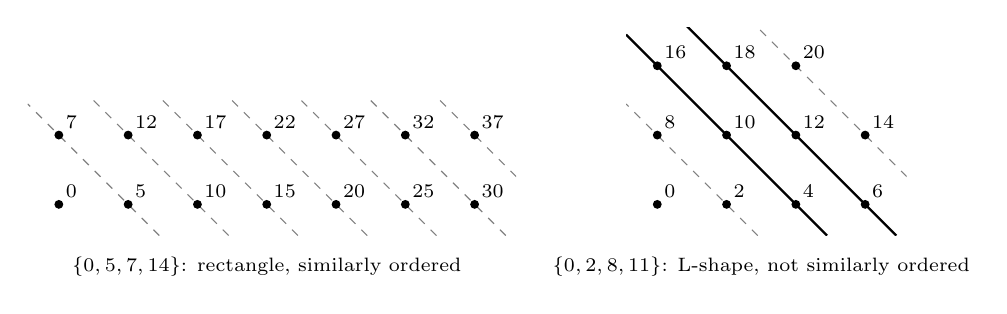
\begin{tikzpicture}[x=0.88cm,y=0.88cm,every node/.style={font=\scriptsize}]
\begin{scope}
\begin{scope}\clip (-0.45,-0.45) rectangle (6.6,1.55);
\foreach \t in {1,...,7} {\draw[gray,dashed] (\t+0.45,-0.45) -- (-0.45,\t+0.45);}
\end{scope}
\foreach \x in {0,...,6} {\foreach \y in {0,1} {
  \pgfmathtruncatemacro{\v}{5*\x+7*\y}
  \fill (\x,\y) circle (1.6pt); \node[above right=-1pt] at (\x,\y) {\v};}}
\node at (3,-0.9) {$\{0,5,7,14\}$: rectangle, similarly ordered};
\end{scope}
\begin{scope}[xshift=7.6cm]
\begin{scope}\clip (-0.45,-0.45) rectangle (3.6,2.55);
\foreach \t in {1,4} {\draw[gray,dashed] (\t+0.45,-0.45) -- (-0.45,\t+0.45);}
\foreach \t in {2,3} {\draw[black,thick] (\t+0.45,-0.45) -- (-0.45,\t+0.45);}
\end{scope}
\foreach \x/\y in {0/0,1/0,2/0,3/0,0/1,1/1,2/1,3/1,0/2,1/2,2/2} {
  \pgfmathtruncatemacro{\v}{2*\x+8*\y}
  \fill (\x,\y) circle (1.6pt); \node[above right=-1pt] at (\x,\y) {\v};}
\node at (1.5,-0.9) {$\{0,2,8,11\}$: L-shape, not similarly ordered};
\end{scope}
\end{tikzpicture}
\caption{Ap\'ery diagrams, each point $(x,y)$ labeled with $a_1x+a_2y$; the lines are the layers $x+y=t$. For $\{0,5,7,14\}$ the values on every layer lie in one interval $(14(q-1),14q]$. For $\{0,2,8,11\}$ the layers $t=2$ and $t=3$ (solid) carry the values $4,10,16$ and $6,12,18$, which cross $11$. Drawn with Ti\emph{k}Z code written by Claude Opus (Anthropic) from the computed Ap\'ery sets.}\label{fig:diagrams}
\end{figure}

\begin{proposition}[Families]\label{prop:families}
\begin{enumerate}
\item[(a)] Let $1<b<d$ and $d=qb+e$, $0\le e<b$. Then $\{0,1,b,d\}$ is CM if and only if $e=0$ or $q+e\ge b$, and then it is similarly ordered.
\item[(b)] $A_0$ is CM and similarly ordered if and only if $d-A_0$ is. In particular every CM set $\{0,a,d-1,d\}$ is similarly ordered.
\item[(c)] A CM set $\{0,a,d-a,d\}$, $0<a<d-a$, is similarly ordered if and only if $d=3$.
\item[(d)] Every set $\{0,a,a+1,d\}$, $a+1<d$, is CM, and it is similarly ordered if and only if $\mathcal D$ is a rectangle or an L-shape with $P-W=1$ or $Q-Z=1$.
\end{enumerate}
\end{proposition}

\begin{proof}
For $n\in\langle a_1,a_2\rangle$ let $\operatorname{len}(n)$ be the least number of parts $a_1,a_2$ with sum $n$. By the proof of Lemma~\ref{lem:diagram}, $A_0$ is CM if and only if $w^{(2)}_{-r}=\operatorname{len}(w^{(1)}_r)d-w^{(1)}_r$ for all $r$. The elements of $S_2$ of class $-r$ avoiding the part $d$ are $\ell'd-(w^{(1)}_r+kd)$ for representations of $w^{(1)}_r+kd$ by $\ell'$ interior parts, with $k\ge0$ by minimality of $w^{(1)}_r$. Hence $A_0$ is CM if and only if
\begin{equation}\label{eq:lambda-test}
\operatorname{len}(w^{(1)}_r+kd)-\operatorname{len}(w^{(1)}_r)\ge k\qquad(0\le r<d,\ k\ge0,\ w^{(1)}_r+kd\in\langle a_1,a_2\rangle).
\end{equation}
(a) Here $\Ap(S_1;d)=[0,d-1]$, and the shortest representation of $n$ uses $\lfloor n/b\rfloor$ parts $b$ and $n\bmod b$ parts $1$, so $\operatorname{len}(n)=\lfloor n/b\rfloor+(n\bmod b)$. Adding $d=qb+e$ raises $\operatorname{len}$ by $q$ if $e=0$. Otherwise it raises it by $q+e$, or by $q+e-b+1$ when the remainder passes $b$. If $q+e\ge b$, every increment is at least $1$ and \eqref{eq:lambda-test} follows. If $0<e$ and $q+e<b$, the element $n=b-e$ of $\Ap(S_1;d)$ violates it, since $n+d=(q+1)b$ and its length rises by $q+e-b+1\le0$. Since $w^{(1)}_r=r$, we have $u_s=1$ for every $s\ge1$, and the pairs $(1,v_s)$ form a chain together with $(0,0)$.
(b) Reflection exchanges the two coordinates of $\mathcal S$, so it preserves the CM property; it exchanges $S_1$ and $S_2$, and with $s'=d-s$ the reflected pairs are $(v_s+1,u_s-1)$ for $s\ne0$. Swapping the coordinates of two pairs and shifting them by the same amounts keeps them comparable or incomparable, so similar ordering is preserved. The second claim follows from (a).
(c) Here reflection fixes the set, so with each pair $(u,v)$, $s\ne0$, the pair $(v+1,u-1)$ occurs on the same layer; comparability forces $u=v+1$, so the layer $u+v$ is odd. For $d>3$ the order ideal $\mathcal D$ has more than three points, while layers $0$ and $1$ hold at most three, hence a point on layer $2$, which is impossible. For $d=3$ the pairs are $(0,0),(1,0),(1,0)$.
(d) Let $b=a+1$. The representation of $n\in\langle a,b\rangle$ with fewest parts has $x(n)=(-n)\bmod b\le a$ parts $a$, so $\operatorname{len}(n)=(n+x(n))/b$, and for $k\ge1$, $\operatorname{len}(n+kd)-\operatorname{len}(n)\ge(kd-a)/b>k-1$ as $d>b$; so \eqref{eq:lambda-test} holds. If both notch dimensions are at least $2$, use Proposition~\ref{prop:shape}. Otherwise each layer is a set of consecutive lattice points (on an L-shape the points of layer $t$ with $x<W$ and those with $x\ge W$ are separated only if $(W,t-W)$ lies in the notch while both groups are nonempty, that is $W+Z\le t\le\min(W+Q-2,P+Z-2)$, a range that is empty when $P-W=1$ or $Q-Z=1$), with consecutive values $at+y$; none of these is a multiple of $d$ for $t>0$, since it would share the residue of $(0,0)$, so the layer lies in one interval $((q-1)d,qd)$.
\end{proof}

The condition in (a) is also the condition under which the cardinality formula of Chen and Yang for $|h\{0,1,b,d\}|$ holds \cite[Cor.~1]{ChenYang2026}, obtained there by the same count of least numbers of parts; the similar-ordering conclusion is not in their statement.

The family $\{0,a,b,2b\}$ of Section~\ref{sec:family} is similarly ordered at $m=b$ (Lemma~\ref{lem:family-residue}) but not always at $m=2b$: $\{0,2,5,10\}$ has $\mathcal D=[0,4]\times[0,1]$, and its layer $4$ has values $8$ and $11$. Theorem~\ref{thm:similar} is a finite arithmetic test from the two Ap\'ery sets; a description of the similarly ordered triples $(a_1,a_2,d)$ by a short list of congruence or continued-fraction conditions is not known (Section~\ref{sec:open}).
